% Options for packages loaded elsewhere
\PassOptionsToPackage{unicode}{hyperref}
\PassOptionsToPackage{hyphens}{url}
%
\documentclass[
]{article}
\usepackage{amsmath,amssymb}
\usepackage{lmodern}
\usepackage{ifxetex,ifluatex}
\ifnum 0\ifxetex 1\fi\ifluatex 1\fi=0 % if pdftex
  \usepackage[T1]{fontenc}
  \usepackage[utf8]{inputenc}
  \usepackage{textcomp} % provide euro and other symbols
\else % if luatex or xetex
  \usepackage{unicode-math}
  \defaultfontfeatures{Scale=MatchLowercase}
  \defaultfontfeatures[\rmfamily]{Ligatures=TeX,Scale=1}
\fi
% Use upquote if available, for straight quotes in verbatim environments
\IfFileExists{upquote.sty}{\usepackage{upquote}}{}
\IfFileExists{microtype.sty}{% use microtype if available
  \usepackage[]{microtype}
  \UseMicrotypeSet[protrusion]{basicmath} % disable protrusion for tt fonts
}{}
\makeatletter
\@ifundefined{KOMAClassName}{% if non-KOMA class
  \IfFileExists{parskip.sty}{%
    \usepackage{parskip}
  }{% else
    \setlength{\parindent}{0pt}
    \setlength{\parskip}{6pt plus 2pt minus 1pt}}
}{% if KOMA class
  \KOMAoptions{parskip=half}}
\makeatother
\usepackage{xcolor}
\IfFileExists{xurl.sty}{\usepackage{xurl}}{} % add URL line breaks if available
\IfFileExists{bookmark.sty}{\usepackage{bookmark}}{\usepackage{hyperref}}
\hypersetup{
  pdftitle={Trapping protocol},
  hidelinks,
  pdfcreator={LaTeX via pandoc}}
\urlstyle{same} % disable monospaced font for URLs
\usepackage[margin=1in]{geometry}
\usepackage{graphicx}
\makeatletter
\def\maxwidth{\ifdim\Gin@nat@width>\linewidth\linewidth\else\Gin@nat@width\fi}
\def\maxheight{\ifdim\Gin@nat@height>\textheight\textheight\else\Gin@nat@height\fi}
\makeatother
% Scale images if necessary, so that they will not overflow the page
% margins by default, and it is still possible to overwrite the defaults
% using explicit options in \includegraphics[width, height, ...]{}
\setkeys{Gin}{width=\maxwidth,height=\maxheight,keepaspectratio}
% Set default figure placement to htbp
\makeatletter
\def\fps@figure{htbp}
\makeatother
\setlength{\emergencystretch}{3em} % prevent overfull lines
\providecommand{\tightlist}{%
  \setlength{\itemsep}{0pt}\setlength{\parskip}{0pt}}
\setcounter{secnumdepth}{-\maxdimen} % remove section numbering
\ifluatex
  \usepackage{selnolig}  % disable illegal ligatures
\fi

\title{Trapping protocol}
\author{}
\date{\vspace{-2.5em}2021-06-26}

\begin{document}
\maketitle

\hypertarget{preparation-for-field-work}{%
\subsection{Preparation for field
work}\label{preparation-for-field-work}}

Before going to the field it's important the following are checked

\begin{enumerate}
\def\labelenumi{\arabic{enumi}.}
\tightlist
\item
  Adequate number of clean and functioning Sherman traps are brought.
  You will need at least \textbf{324} to set up the correct number so
  please bring some extra.
\item
  Enough sample pots for rodent specimens
\item
  Spare batteries for GPS devices
\item
  Battery packs if possible for the electronic tablets
\item
  Working portable freezer that can be stored at Panguma Hospital Lab
\item
  Paper copies of the data entry form in case the pads stop working
\end{enumerate}

\begin{figure}
\centering
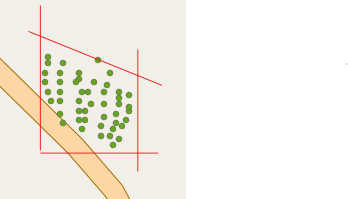
\includegraphics{figures/grid.png}
\caption{For example this was the grid we set up for trap site 5 at
Lalehun}
\end{figure}

\hypertarget{finding-the-trap-sites}{%
\subsection{Finding the trap sites}\label{finding-the-trap-sites}}

Using the GPS device (GPS MAP65) to find the study sites.

The coordinates of the corners of the study grids are below. To find
them you can use the GPS.

First turn on the device and press the find button on the front above
mark. Use the direction buttons to select Coordinates and press enter.
This takes to a page that asks you to enter the location. The left and
right arrows at the bottom of the screen move across the numbers you can
control what is highlighted using the directional buttons and enter
selects. This will then produce a purple line that will guide you to the
coordinates. Tie some ribbon to a plant to identify this corner of the
grid and then perform the same for the 3 other corners.

\includegraphics{protocol_files/figure-latex/traps-1.pdf}

\hypertarget{lalehun}{%
\subsubsection{Lalehun}\label{lalehun}}

We have set up \textbf{six} sites in Lalehun. Each site represents a
grid that we set lines of traps in. Each line is 7 traps.

For each of the below grids there are coordinates for the corners of the
grid. Try and set up lines of traps within the grids so it would be
easier if you find the corners first

\begin{enumerate}
\def\labelenumi{\arabic{enumi}.}
\tightlist
\item
  \textbf{Grid 1}: Edge of the village

  \begin{itemize}
  \tightlist
  \item
    Closest to the village = 8 11.801 N and 11 4.767 W
  \item
    Furthest from the village = 8 11.782 N and 11 4.742 W
  \item
    8 11.781 N and 11 4.775 W
  \item
    9 11.769 N and 11 4.758 W
  \end{itemize}
\item
  \textbf{Grid 2}: Within and near a wet rice field

  \begin{itemize}
  \tightlist
  \item
    Closest to the village = 8 11.921 N and 11 4.771 W
  \item
    8 11.94 N and 11 4.758 W
  \item
    Furthest in the field = 8 11.923 N and 11 4.727 W
  \item
    8 11.908 and 11 4.739 W
  \end{itemize}
\item
  \textbf{Grid 3}: Split into two, one part on the banana field and
  fallow land, the other on the banana field and pineapple garden

  \begin{itemize}
  \tightlist
  \item
    Near the compound = 8 11.9417 N and 11 4.811 W
  \item
    In the fallow land = 8 11.92 N and 11 4.822 W
  \item
    By the water store = 8 11.967 N and 11 4.826 W
  \item
    In the fallow land = 8 11.953 N and 11 4.838 W
  \end{itemize}
\item
  \textbf{Grid 4}: Long term fallow land

  \begin{itemize}
  \tightlist
  \item
    Closest to the road = 8 11.644 N and 11 4.699 W
  \item
    Across the hill = 8 11.687 N and 11 4.696 W
  \item
    Up the hill = 8 11.644 N and 11 4.681 W
  \item
    Up the hill furthest from the road = 8 11.687 N and 11 4.68 W
  \end{itemize}
\item
  \textbf{Grid 5}: Cassava plantation

  \begin{itemize}
  \tightlist
  \item
    Close to the road = 8 11.619 N and 11 4.811 W
  \item
    Down the hill along the road = 8 11.633 N and 11 4.831 W
  \item
    Into the field = 8 11.647 N and W 11 4.832 W
  \item
    8 11.635 N and 11 4.806 W
  \end{itemize}
\item
  In 3 lines through the village

  \begin{itemize}
  \tightlist
  \item
    Line 1 beginning = 8 11.911 N and 11 4.797 W
  \item
    Line 1 end = 8 11.819 N and 11 4.79 W
  \item
    Line 2 beginning = 8 11.888 N and 11 4.822 W
  \item
    Line 2 end = 8 11.82 N and 11 4.802 W
  \item
    Line 3 beginning = 8 11.872 N and 11 4.828 W
  \item
    Line 3 end = 8 11.809 N and 11 4.818 W
  \end{itemize}
\item
  \textbf{Within houses}

  \begin{itemize}
  \tightlist
  \item
    4 traps per home
  \end{itemize}
\end{enumerate}

We will add another ``site'' which will be traps within the houses. For
the traps in the houses it is important to note what the room is used
for, the type of material the house is made from and the type of roof.

For Lalehun we want to have traps in homes from across the village.
Please try and make sure that traps are placed in homes from as many as
the squares of \textbf{Figure 2} as possible. You will also need to
record how many houses you asked to place traps in and how many said no.
There is a separate \textbf{Indoor} sheet to record this on.

\hypertarget{seilama}{%
\subsubsection{Seilama}\label{seilama}}

Is positioned in a relatively forested area South West of Panguma. There
is significant agricultural activity with fallow, clearance and burning
practices used.

We have set up \textbf{six} sites in Seilama.

\begin{enumerate}
\def\labelenumi{\arabic{enumi}.}
\tightlist
\item
  \textbf{Grid 1}: Palm plantation, near the village and main road

  \begin{itemize}
  \tightlist
  \item
    Close to the main road = 8 7.325 N and 11 11.539 W
  \item
    Down the road away from the village = 8 7.375 N and 11 11.511 W
  \item
    8 7.375 N and 11 11.535
  \item
    Set this corner yourself
  \end{itemize}
\item
  \textbf{Grid 2}: Cacao and Coffee plantation

  \begin{itemize}
  \tightlist
  \item
    Close to the village = 8 7.378 N and 11 11.649 W
  \item
    Along the stream = 8 7.4 N and 11 11.643 W
  \item
    8 7.413 N and 11 11.653 W
  \item
    Away from the village = 8 7.384 N and 11 11.67 W
  \end{itemize}
\item
  \textbf{Grid 3}: Recently harvested dry rice field

  \begin{itemize}
  \tightlist
  \item
    Close to the village = 8 7.424 N and 11 11.657 W
  \item
    Along the ravine = 8 7.446 N and 11 11.66 W
  \item
    8 7.467 N and 11 11.672 W
  \item
    8 7.443 N and 11 11.685 W
  \end{itemize}
\item
  \textbf{Grid 4}: Wet rice plantation

  \begin{itemize}
  \tightlist
  \item
    Closest to the village = 8 7.234 N and 11 11.651 W
  \item
    Furthest from the village = 8 7.22 N and 11 11.669 W
  \item
    Into the field = 8 7.255 N and 11 11.673 W
  \item
    8 7.234 N and 11 11.678 W
  \item
    Line outside of grid beginning = 8 7.258 N and 11 11.619 W
  \item
    Line outside of grid end = 8 7.258 N and 11 11.619 W
  \end{itemize}
\item
  \textbf{Grid 5}: Disturbed forest, long term fallow

  \begin{itemize}
  \tightlist
  \item
    Closest to the village = 8 7.413 N and 11 11.871 W
  \item
    Away from the village = 8 7.428 N and 11 11.884 W
  \item
    8 7.441 N and 11 11.861 W
  \item
    8 7.43 N and 11 11.849 W
  \end{itemize}
\item
  Within the village, outside of houses, two lines of 7 within the
  village

  \begin{itemize}
  \tightlist
  \item
    Set in a ring around the village
  \item
    Line 1 beginning = 8 7.307 N and 11 11.625 W
  \item
    Line 1 end = 8 7.357 N and 11 11.624 W
  \item
    Line 2 beginning = 8 7.31 N and 11 11.6 W
  \item
    Line 2 end = 8 7.362 N and 11 11.611 W
  \end{itemize}
\item
  \textbf{Within home}
\end{enumerate}

Seilama is a much smaller village so just try and make sure that you
have good coverage of the different areas of the village when setting
the traps in houses.

\hypertarget{bambawo}{%
\subsubsection{Bambawo}\label{bambawo}}

Bambawo was selected due to its proximity to the national park and
relatively heavily forested areas of Eastern Province while being on the
outskirts of Kenema.

Four sites have been established in the village. We were missing traps
for the first visit so two further trap sites will be established on the
the next visit. Traps across the village and within the houses will be
placed starting at visit 2.

\begin{enumerate}
\def\labelenumi{\arabic{enumi}.}
\tightlist
\item
  \textbf{Grid 1}: Far forest site. Previously used by mining company.
  Remains of accomodation houses for miners in the area. Forest
  currently used for animal trapping, nil significant disturbance. +
\item
  \textbf{Grid 2}: Rice farm on hillside recently cleared and burned.
\item
  \textbf{Grid 3}: Old quarry site. Open mining now not significantly
  used. Low lying shrub surrounds
\item
  \textbf{Grid 4}: Mixed used agricultural land near the village.
  Currently grain and banana.
\end{enumerate}

\hypertarget{data-collection-process}{%
\subsection{Data collection process}\label{data-collection-process}}

\hypertarget{direct-odk-entry-preferred}{%
\subsubsection{\texorpdfstring{Direct ODK entry
\textbf{(Preferred)}}{Direct ODK entry (Preferred)}}\label{direct-odk-entry-preferred}}

There are three forms you can access through ODK connect on your mobile
phone or the study team tablets. The forms once saved will automatically
be sent to the ODK server once they can connect to the internet. There
is a sim card in the tablet that can be loaded with credit.

\begin{enumerate}
\def\labelenumi{\arabic{enumi}.}
\tightlist
\item
  site\_setup\_v2: This sheet is completed for each site on the first
  day of trapping. It is important to ensure you correctly write the
  trap number and it's coordinates. If you make any errors you can edit
  the file or notify Dianah/David and they can amend it. You will
  describe each site, the habitat and surroundings of each trap and the
  coordinates for each trap. Photos can be taken if you are having
  difficulty completing the questions.
\item
  trap\_check\_v1: This sheet is used to collect information about the
  number of traps missing \textbf{bait}, \textbf{have been sprung shut}
  or contain \textbf{rodents} the next morning. It may be easier to note
  the traps on a piece of paper first and then to enter the data into
  ODK.
\item
  rodent\_v1: This sheet is used to collect information about the
  trapped rodent. The most important parts of this are to ensure that
  the trap number and rodent number are correct. The trap number is
  important to know where the rodent came from. The rodent number should
  be made by putting the number of the visit, then the 3 letters of the
  village and then the number this rodent is for this visit. For
  example: + The 12th rodent trapped in the 2nd visit in Seilama would
  be 2SEI-012 + The 3rd rodent trapped on the 1st visit in Bambawo would
  be 1BAM-003
\end{enumerate}

\hypertarget{data-entry-sheets}{%
\subsubsection{Data entry sheets}\label{data-entry-sheets}}

The \textbf{Trap site setup} sheet needs to be completed once for each
trap site (the grid of 49 traps) once during the study visit for all of
the sites that are setup (so 7 including the indoor traps). I expect 7
completed forms from each village. Please try and be as accurate as
possible with the GPS coordinates.

The \textbf{Trap check} sheet needs to be completed for each trap site
for each study night.

The \textbf{Rodent} sheet needs to be completed for each rodent that has
been trapped.

The \textbf{Indoor} sheet only needs to be completed once for each set
of traps placed indoors, so once per village.

\end{document}
